\documentclass[a4paper]{oblivoir}
\usepackage{amsmath,amssymb,kotex,mdframed,paralist}
\usepackage{fapapersize}
\usefapapersize{210mm,297mm,20mm,*,20mm,*}

\usepackage{tabto,pifont}
\TabPositions{0.2\textwidth,0.4\textwidth,0.6\textwidth,0.8\textwidth}

%%% 객관식 선지
\newcommand\one{\ding{172}}
\newcommand\two{\ding{173}}
\newcommand\three{\ding{174}}
\newcommand\four{\ding{175}}
\newcommand\five{\ding{176}}
\usepackage{tabto,pifont}
%\TabPositions{0.2\textwidth,0.4\textwidth,0.6\textwidth,0.8\textwidth}

\newcommand\taba[5]{\par\noindent
\one\:{#1}
\tabto{0.2\textwidth}\two\:\:{#2}
\tabto{0.4\textwidth}\three\:\:{#3}
\tabto{0.6\textwidth}\four\:\:{#4}
\tabto{0.8\textwidth}\five\:\:{#5}}

\newcommand\tabb[5]{\par\noindent
\one\:{#1}
\tabto{0.33\textwidth}\two\:\:{#2}
\tabto{0.67\textwidth}\three\:\:{#3}\medskip\par\noindent
\four\:\:{#4}
\tabto{0.33\textwidth}\five\:\:{#5}}

\newcommand\tabc[5]{\par\noindent
\one\:{#1}
\tabto{0.5\textwidth}\two\:\:{#2}\medskip\par\noindent
\three\:\:{#3}
\tabto{0.5\textwidth}\four\:\:{#4}\medskip\par\noindent
\five\:\:{#5}}

\newcommand\tabd[5]{\par\noindent
\one\:{#1}\medskip\par\noindent
\two\:\:{#2}\medskip\par\noindent
\three\:\:{#3}\medskip\par\noindent
\four\:\:{#4}\medskip\par\noindent
\five\:\:{#5}}

\usepackage{graphicx}

%\pagestyle{empty}

%%% Counters
\newcounter{num}

%%% Commands
\newcommand{\prob}[1]
{\bigskip\bigskip\noindent\refstepcounter{num}\textbf{문제 \arabic{num})} #1\par\noindent}

\newcommand\pb[1]{\ensuremath{\fbox{\phantom{#1}}}}

\newcommand\ba{\ensuremath{\:|\:}}

\newcommand\vs[1]{\par\vspace{40pt}}

\newcommand\an[1]{\bigskip\par\noindent\textbf{문제 #1)}\par\noindent}

%%% Meta Commands
\let\oldsection\section
\renewcommand\section{\clearpage\oldsection}

\let\emph\textsf

\begin{document}
\begin{center}
\LARGE태희, 미니테스트 02
\end{center}
\begin{flushright}
날짜 : 2018년 \(\pb3\)월 \(\pb{10}\)일 \(\pb{월}\)요일
,\qquad
제한시간 : \pb{17년}분
,\qquad
점수 : \pb{20} / \pb{20}
\end{flushright}

%
\prob{
두 집합 \(X=\{1,2,3\}\), \(Y=\{1,2,3,4\}\)에 대하여 함수 \(f:X\to Y\)가 \(x_1<x_2\)이면 \(f(x_1)<f(x_2)\)를 만족시킬 때, 함수 \(f\)의 개수는?
(단, \(x_1\in X\), \(;x_2\in X\))
}
\taba23456
\vs

%
\prob{
두 집합  \(X=\{1,2,3,4,5\}\), \(Y=\{y\ba1\le y\le10\text{인 자연수}\}\)에 대하여 \(f(3)=5\)일 때, 집합 \(X\)의 임의의 두 원소 \(x_1\), \(x_2\)에 대하여 \(x_1<x_2\)이면 \(f(x_1)<f(x_2)\)를 만족시키는 함수 \(f\)의 개수를 구하여라.
}
\vs

\noindent
\begin{minipage}{.8\textwidth}
%
\prob{
오른쪽 그림과 같이 원 위에 8개의 점이 같은 간격으로 놓여있다.
주어진 점을 이어서 만들 수 있는 직선의 개수는?
}
\taba{22}{24}{26}{28}{30}
\end{minipage}
\begin{minipage}{.2\textwidth}
\centering
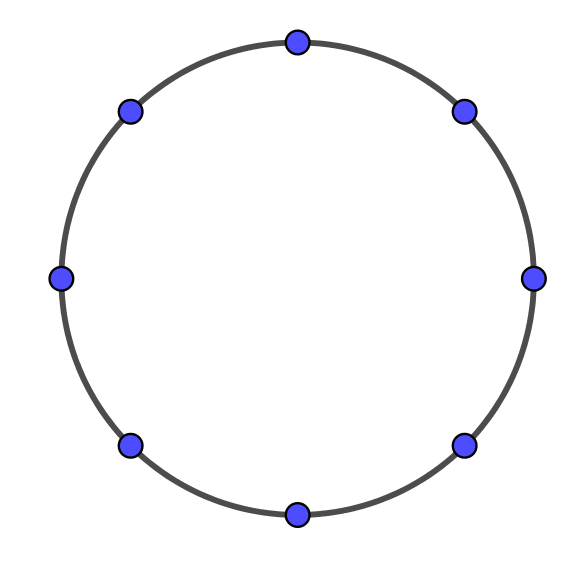
\includegraphics[width=.7\textwidth]{eightpoints}
\end{minipage}
\vs

\noindent
\begin{minipage}{.8\textwidth}
%
\prob{오른쪽 그림과 같은 정육각형의 대각선의 개수는?}
\taba6789{10}
\end{minipage}
\begin{minipage}{.2\textwidth}
\centering
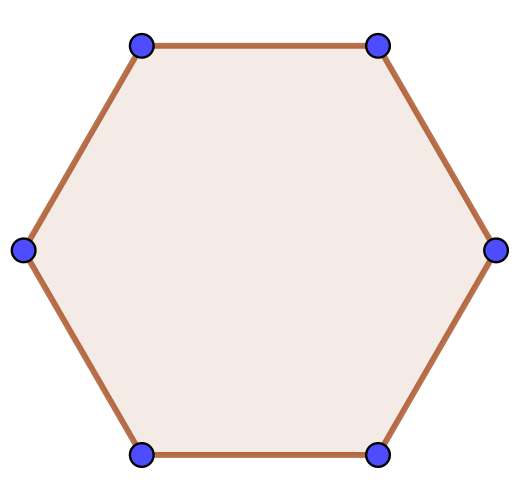
\includegraphics[width=.7\textwidth]{hexagon}
\end{minipage}
\vs

%
\prob{볼록 12각형의 서로 다른 대각선의 교점의 개수의 최댓값을 구하여라.}
\vs

\noindent
\begin{minipage}{.8\textwidth}
%
\prob{
오른쪽 그림과 같이 반원 위에 7개의 점이 있다.
이 중 세 점을 꼭짓점으로 하는 삼각형의 개수는?
\taba{30}{31}{32}{33}{34}
}
\end{minipage}
\begin{minipage}{.2\textwidth}
\centering
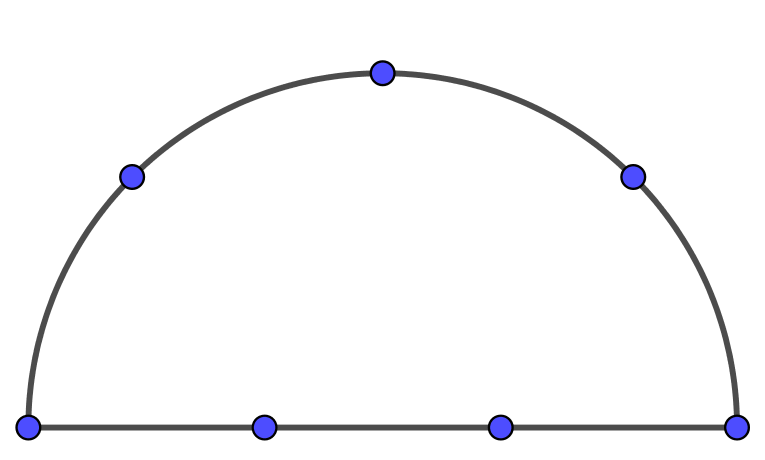
\includegraphics[width=.7\textwidth]{sevenpoints}
\end{minipage}
\vs

%
\prob{서로 다른 8개의 구슬을 4개, 4개로 나누는 방법의 수를 \(a\)라고 하고, 5개, 3개로 나누는 방법의 수를 \(b\)라고 할 때, \(b-a\)의 값을 구하여라.}
\vs

%
\prob{
6개의 원소로 이루어진 집합  \(\{a,b,c,d,e,f\}\)의 원소들을 2개, 2개, 2개로 분할하는 방법의 수를 구하여라.}
\taba{5}{10}{15}{25}{30}

%
\prob{다음의 문장이나 식들 중 참인 문장에는 `T'를, 거짓인 문장에는 `F'를 써넣으시오.}
\begin{enumerate}[(1)]
\item
\(n\)이 짝수이면 \(y=x^n\)은 기함수이다.
\item
\(4\)의 제곱근 중 실수인 것은 한 개이다.
\item
\(8\)의 세제곱근 중 실수인 것은 한 개이다.
\item
\(16\)의 네제곱근 중 실수인 것은 한 개이다.
\item
\(a<0\)이면 \(\sqrt[3]a<0\)이다.
\item
\(a>0\)이면 \(\sqrt[4]a>0\)이다.
\item
\(\sqrt[3]5\times\sqrt[3]{25}=5\)
\item
\(\sqrt{(-3)^2}=-3\)
\item
\(\sqrt[3]{(-3)^3}=-3\)
\item
\(\sqrt[4]{(-3)^4}=-3\)
\item
\(\sqrt{-2}=-\sqrt2\)
\item
\(\sqrt[3]{-2}=-\sqrt[3]2\)
\item
\(\sqrt[4]{-2}=-\sqrt[4]2\)
\item
\((\sqrt[5]2)^{10}=32\)
\item
\(\displaystyle\frac{\sqrt[3]{243}}{\sqrt[3]9}=3\)
\item
\(\sqrt[5]{\sqrt[3]{7^{15}}}=1\)
\end{enumerate}

%
\prob{}
\(\displaystyle \sqrt{a\sqrt{a\sqrt{a\sqrt a}}}=a^x\)일 때, \(x\)의 값을 구하여라.
\end{document}